
\documentclass[conference]{IEEEtran}

\ifCLASSINFOpdf
  % \usepackage[pdftex]{graphicx}
  % declare the path(s) where your graphic files are
  % \graphicspath{{../pdf/}{../jpeg/}}
  % and their extensions so you won't have to specify these with
  % every instance of \includegraphics
  % \DeclareGraphicsExtensions{.pdf,.jpeg,.png}
\else
  % or other class option (dvipsone, dvipdf, if not using dvips). graphicx
  % will default to the driver specified in the system graphics.cfg if no
  % driver is specified.
  % \usepackage[dvips]{graphicx}
  % declare the path(s) where your graphic files are
  % \graphicspath{{../eps/}}
  % and their extensions so you won't have to specify these with
  % every instance of \includegraphics
  % \DeclareGraphicsExtensions{.eps}
\fi



% correct bad hyphenation here
\pagestyle{headings}

% Note that the line below could be modified to suit a
% particular system since the "geometry" package behaves
% differently in Unix, Windows and Mac, especially for the
% top margins.
% Adjust the parameter "top" (measuring the height of the
% space allocated to a header) and "headsep" (measuring
% the distance from the bottom of the header to the
% first line of text.
\usepackage[top=1.3in,left=1.5in,bottom=1in,right=1in,headsep=0.5in]{geometry}

\usepackage{setspace}
\onehalfspacing
%\doublespacing

% Headers and footers for thesis
\usepackage{fancyhdr}

\markboth{}{}
\newcommand\startchapter[1]{\chapter{#1}\thispagestyle{myheadings}}
\newcommand\startappendix[1]{\chapter{#1}\thispagestyle{myheadings}}
\newcommand\startfirstchapter[1]{\chapter{#1}}

% Manual addition of section to Table of Contents
\newcommand\TOCadd[1]{\newpage\phantomsection\addcontentsline{toc}{chapter}{#1}}

% Float Customization
\renewcommand{\floatpagefraction}{0.01}

% Customization of Tables of Contents and List of Figures/Tables
\usepackage{tocloft}
\renewcommand\cfttabpresnum{Table\ }
\renewcommand\cfttabnumwidth{0.75in}
\renewcommand\cftfigpresnum{Figure\ }
\renewcommand\cftfignumwidth{0.80in}
\newcommand{\HRule}{\rule{\linewidth}{0.5mm}}


% Long Table and decimal aligned columns
\usepackage{dcolumn}
\usepackage{longtable}

% Mathematics support
\usepackage{amsmath}
\usepackage{amsthm}
\usepackage{amssymb}


% Text Control
\usepackage{xspace}
\usepackage{textcase}

% Graphics
\usepackage{wasysym}
\usepackage{graphics}
\usepackage{graphicx}   % A package to allow insertion of
                        % external image files


%\usepackage{cite}
\usepackage[backend=bibtex,style=numeric, sorting=none]{biblatex}
\usepackage[acronym]{glossaries}
\usepackage{nomencl}
\usepackage{array}
\usepackage{mathtools}
\usepackage{multicol}
\usepackage[flushleft]{threeparttable}
\usepackage{amsmath}
\usepackage{listings}
\usepackage{color}
\usepackage{graphicx}
\usepackage{caption}
\usepackage{subcaption}
\usepackage{siunitx}
\usepackage{multirow}
\usepackage{csquotes}
\let\labelindent\relax
\usepackage{enumitem}
\setlist{nolistsep}
\usepackage{stfloats}
\newcolumntype{C}{>{$}c<{$}} % math-mode version of "l" column type
%\loadglsentries{Utils/Glossary}
\makenomenclature
\renewcommand{\nomname}{List of Symbols}
\newcommand{\Xilinx}{\textit{\gls{Xilinx}}~}
\newcommand{\ConditionSize}{\footnotesize}

\newcommand{\Name}{\acrshort{FPGA} Trojan Detector}
\newcommand{\NameNoPeriod}{\Name~}
\newcommand{\WebName}{Hardware Trojan System}
\newcommand{\WebNameNoPeriod}{\WebName~}

\newcommand{\Swing}{\textit{Swing}~}
\newcommand{\SwingEnd}{\textit{Swing}}
\newcommand{\RapidSmith}{\textit{RapidSmith}~}
\DeclarePairedDelimiter\ceil{\lceil}{\rceil}
\DeclarePairedDelimiter\floor{\lfloor}{\rfloor}
\definecolor{dkgreen}{rgb}{0.1,0.5,0}
\definecolor{gray}{rgb}{0.5,0.5,0.5}
\definecolor{mauve}{rgb}{0.58,0,0.82}

\lstset{frame=tb,
	aboveskip=1mm,
	belowskip=1mm,
	showstringspaces=false,
	columns=flexible,
	basicstyle={\small\ttfamily},
	numbers=none,
	numberstyle=\tiny\color{gray},
	keywordstyle=\color{blue},
	commentstyle=\color{dkgreen},
	stringstyle=\color{mauve},
	breaklines=true,
	breakatwhitespace=true,
	tabsize=3
}
\newenvironment{conditions}
{\par\vspace{\abovedisplayskip}\noindent\begin{tabular}{>{$}l<{$} @{${}={}$} l}}
	{\end{tabular}\par\vspace{\belowdisplayskip}}
\addbibresource{UvicThesis.bib} 
\begin{document}
%
% paper title
% can use linebreaks \\ within to get better formatting as desired
\title{Automated Hardware Trojan Detection in FPGAs}


% author names and affiliations
% use a multiple column layout for up to three different
% affiliations
\author{\IEEEauthorblockN{Nicholas Houghton, Samer Moein, and Fayez Gebali}
	\IEEEauthorblockA{Department of Electrical and Computer Engineering\\
		University of Victoria\\
		P.O. Box 1700 STN CSC\\
		Victoria, B.C. V8W 2Y2\\
		Email: \{nhoughto, samerm, fayez\}@uvic.ca}}

% conference papers do not typically use \thanks and this command
% is locked out in conference mode. If really needed, such as for
% the acknowledgment of grants, issue a \IEEEoverridecommandlockouts
% after \documentclass

% for over three affiliations, or if they all won't fit within the width
% of the page, use this alternative format:
% 
%\author{\IEEEauthorblockN{Michael Shell\IEEEauthorrefmark{1},
%Homer Simpson\IEEEauthorrefmark{2},
%James Kirk\IEEEauthorrefmark{3}, 
%Montgomery Scott\IEEEauthorrefmark{3} and
%Eldon Tyrell\IEEEauthorrefmark{4}}
%\IEEEauthorblockA{\IEEEauthorrefmark{1}School of Electrical and Computer Engineering\\
%Georgia Institute of Technology,
%Atlanta, Georgia 30332--0250\\ Email: see http://www.michaelshell.org/contact.html}
%\IEEEauthorblockA{\IEEEauthorrefmark{2}Twentieth Century Fox, Springfield, USA\\
%Email: homer@thesimpsons.com}
%\IEEEauthorblockA{\IEEEauthorrefmark{3}Starfleet Academy, San Francisco, California 96678-2391\\
%Telephone: (800) 555--1212, Fax: (888) 555--1212}
%\IEEEauthorblockA{\IEEEauthorrefmark{4}Tyrell Inc., 123 Replicant Street, Los Angeles, California 90210--4321}}




%%%%%%%%%%%%%%%%%%%%%%%%%%%%%%%%%%%%%%%%%%%%%%%%%%%%%%%%%
%To compile glossary and acronyms run following sequence under Tools
%Commands -> pdfLatex
%User -> MakeGlossaries
%Commands -> Make Index
%Commands -> pdfLatex
%Build
%%%%%%%%%%%%%%%%%%%%%%%%Acronyms%%%%%%%%%%%%%%%%%%%%%%%%%
\newacronym{FPGA}{FPGA}{Field Programmable Gate-Array}
\newacronym{FPGAs}{FPGA}{Field Programmable Gate-Arrays}
\newacronym{CL}{CL}{Configurable Logic}
\newacronym{ASIC}{ASIC}{Application Specific Integrated Circuit}
\newacronym{HDL}{HDL}{Hardware Description Language}
\newacronym{ISE}{ISE}{Integrated Synthesis Environment}
\newacronym{IOB}{IOB}{Input-Output Block}
\newacronym{CLB}{CLB}{Configurable Logic Block}
\newacronym{IOBs}{IOBs}{Input-Output Blocks}
\newacronym{CRC}{CRC}{Cyclic Redundancy Check}
\newacronym{CLBs}{CLBs}{Configurable Logic Blocks}
\newacronym{IOI}{IOI}{Input-Output Interconnect}
\newacronym{IOIs}{IOIs}{Input-Output Interconnects}
\newacronym{IP}{IP}{Intelectual Property}
\newacronym{RO}{RO}{Ring Oscillator}
\newacronym{ROs}{RO}{Ring Oscillators}
\newacronym{LUT}{LUT}{Look-up Table}
\newacronym{IR}{IR}{Interconnect Resources}
\newacronym{SM}{SM}{Switching Matrix}
\newacronym{PIP}{PIP}{Programmable-Interconnect-Points}
\newacronym{XDL}{XDL}{\Xilinx Design Language}
\newacronym{RDB}{RDB}{Readback File}
\newacronym{MSD}{MSD}{The mask file used to hide undesirable configuration information}
\newacronym{DFF}{DFF}{D Flip-Flop}
\newacronym{TCL}{TCL}{Tool Command Line}
\newacronym{JTAG}{JTAG}{Joint Test Action Group}
\newacronym{SRL}{SRL}{Shift Right Left Module}
\newacronym{RAM}{RAM}{Random Access Memory}
\newacronym{LL}{LL}{Logic Allocation File}
\newacronym{RBB}{RBB}{Repeatable Building Blocks}
\newacronym{RBA}{RBA}{Readback ASCII}
\newacronym{RTL}{RTL}{Registry Transfer Level}
\newacronym{TV}{TV}{Test Vectors}
\newacronym{XOR}{XOR}{Exclusive OR}
\newacronym{XNOR}{XNOR}{Exclusive NOR}
\newacronym{UUT}{UUT}{Unit Under Test}
\newacronym{PROM}{PROM}{Programmable Read-Only Memory}
\newacronym{GUI}{GUI}{Graphical User-Interface}
\newacronym{EDIF}{EDIF}{Electronic Data Interchange Format}
\newacronym{NCF}{NCF}{Netlist Constraints File}
\newacronym{UI}{UI}{User-Interface}
\newacronym{UIs}{UI}{User-Interfaces}
\newacronym{DCM}{DCM}{Digital Clock Managers}
\newacronym{ROM}{ROM}{Read-Only Memory}
\newacronym{BEL}{BEL}{Basic Element}
\newacronym{ISCAS}{ISCAS}{IEEE International Symposium on Circuits and Systems}
\newacronym{UCF}{UCF}{User Constraint File}
\newacronym{API}{API}{Application Programming Interface}
\newacronym{APIs}{API}{Application Programming Interfaces}
\newacronym{CAD}{CAD}{Computer Aided Design}
\newacronym{IO}{IO}{Input-Output}
\newacronym{BRAM}{BRAM}{Block \acrlong{RAM}}
\newacronym{SRAM}{SRAM}{Static \acrlong{RAM}}
\newacronym{CMD}{CMD}{Command Register}
\newacronym{WCFG}{WCFG}{CMD Write Packet Data}
\newacronym{MSK}{MSK}{Readback Mask File}
\newacronym{appName}{\textit{F-TRAP}}{\acrshort{FPGA} Trojan Recognition and Parsing}
\newacronym{FLR}{FLR}{Frame Length Register}
\newacronym{IC}{IC}{Integrated Circuit}
\newacronym{ICs}{IC}{Integrated Circuits}
\newacronym{PLD}{PLD}{Programmable Logic Device}
\newacronym{PLDs}{PLD}{Programmable Logic Devices}
\newacronym{ERAI}{ERAI}{Electronic Resellers Association International}
\newacronym{BA}{BA}{Block Address}
\newacronym{GCLK}{GCLK}{Global Clock}
\newacronym{PC}{PC}{Personal Computer}
\newacronym{BYU}{BYU}{Brigham Young University}
%%%%%%%%%%%%%%%%%%%%%%%%Glossary Entries%%%%%%%%%%%%%%%%%
\newglossaryentry{log}{name={log},description={A log file generated by XST}}
\newglossaryentry{Bitstream}{name={Bitstream},description={The sequence of one and zeroes which makes up the configuration data}}
\newglossaryentry{Bit}{name={Bit},description={The binary file containing the configuration data for the implementation}}
\newglossaryentry{Vivado}{name={Vivado},description={The Integrated Development Environment Used Exclusively for 7-series FPGAs}}
\newglossaryentry{Xilinx}{name={Xilinx},description={an American technology company, primarily a supplier of programmable logic devices. It is known for inventing the field-programmable gate array (FPGA) and as the first semiconductor company with a fabless manufacturing model.}}
\newglossaryentry{Readback}{name={Readback},description={A feature in all \Xilinx FPGAs where by the current state of the \gls{gateArray} is stored in the configuration memory to be read by the user via the JTAG port}}
\newglossaryentry{SelectMap}{name={SelectMap},description={A \Xilinx device configuration mode which allows for the programming of multiple devices in parallel}}
\newglossaryentry{golden}{name={Golden},description={The clean, untampered version of the synthesis files generated by XST}}
\newglossaryentry{target}{name={Target},description={The generated files from devices received from the third-party fabrication house}}
\newglossaryentry{Library}{name={\textit{Library}},description={The list of absolute addresses for all components in a \gls{gateArray}}}
\newglossaryentry{NGC}{name={NGC},description={The NGC file is a netlist that contains both logical design data and constraints. The NGC file takes the place of both \acrfull{EDIF} and \acrfull{NCF} files}}
\newglossaryentry{Plan Ahead}{name={Plan Ahead},description={Software provided by \Xilinx for RTL to \gls{Bitstream} design flow management}}
\newglossaryentry{RAM16}{name={RAM16},description={\acrshort{LUT} used as a 16x1 memory unit}}
\newglossaryentry{SRL16}{name={SRL16},description={\acrshort{LUT} used as a 16-bit shift register}}
\newglossaryentry{SLICEM}{name={SLICEM},description={A component of a \acrshort{CLB} in the Spartan-3E family of \acrshort{FPGA}s capable of both logic and memory functions}}
\newglossaryentry{SLICEL}{name={SLICEL},description={A component of a \acrshort{CLB} in the Spartan-3E family of \acrshort{FPGA}s capable of only logic functions}}
\newglossaryentry{sch2hdl}{name={sch2hdl},description={used to convert schematic designs to \gls{HDL}. This stage is optional as many choose to develop directly in \acrshort{HDL}}}
\newglossaryentry{XST}{name={XST},description={\gls{Xilinx} Synthesis Tools, a package that parses, optimizes and compiles the \acrshort{HDL} code.}}
\newglossaryentry{ngdbuild}{name={ngdbuild},description={A tool used to build a NETLIST.}}
\newglossaryentry{MAP}{name={MAP},description={A \gls{Xilinx} tool used to calculate the optimal routing for the finalized design.}}
\newglossaryentry{PAR}{name={PAR},description={used to place and route the design in the specific \Xilinx device.}}
\newglossaryentry{trce}{name={trce},description={used to perform timing and performance analysis.}}
\newglossaryentry{Bitgen}{name={Bitgen},description={The final stage used to generate the configuration \gls{Bitstream} which will configure the device.}}
\newglossaryentry{xdl2ndc}{name={xdl2ndc},description={A command line tool used to convert between the non human-readable ndc netlist format and the human readable \acrshort{XDL} format.}}
\newglossaryentry{thread}{name={thread},description={The smallest sequence of programmed instructions that can be managed independently by a scheduler, which is typically a part of the operating system.}}
\newglossaryentry{Group}{name={Group},description={A collection of columns of 1-bit wide components in an FPGA}}
\newglossaryentry{FragementMatrix}{name={Fragement Matrix},description={A conceptual interpretation of the architecture of an FPGA where by it is imagined as a matrix of 1-bit configurable components}}
\newglossaryentry{QT}{name={QT},description={ a cross-platform application framework that is widely used for developing application software that can be run on various software and hardware platforms. It provides easy to use \acrshort{UI} design tools and features used for this project.~\cite{QT}}}
\newglossaryentry{Boost}{name={Boost},description={ a set of libraries for the C++ programming language that provide support for tasks and structures such as linear algebra, pseudorandom number generation, multithreading, image processing, regular expressions, and unit testing.~\cite{boostLibrary}}}
\newglossaryentry{winAPI}{name={Windows \gls{API}},description={Windows API or WinAPI is a core set of Microsoft's \acrshort{API}s available within the Windows Operating System. It provides basic \acrshort{UI}, Environment handling, data access and storage utilities and more.~\cite{windowsAPI}}}
\newglossaryentry{Fragment}{name={Fragment},description={A 1-bit configurable component of an FPGA. Fragments do not exist however they are used as a conceptual aid to improve understanding of configuration process.}}
\newglossaryentry{gateArray}{name={Gate Array},description={The primary structure of an \gls{FPGA} device. Composed of a regular arrangement of logic gates.}}
\newglossaryentry{positionMedian}{name={Position Median},description={The computed center of an \acrshort{FPGA} design}}
\newglossaryentry{scatterScore}{name={Scatter Score},description={A numeric representation of the clustering of a design}}
% make the title area
\maketitle


\begin{abstract}
%\boldmath
Electronics have become such a staple in modern life that we are just as affected by their vulnerabilities as they are.
Ensuring that the processors that control them are secure is paramount to our intellectual safety, our financial safety, our privacy, and even our personal safety.
The market for integrated circuits is steadily being consumed by a reconfigurable type of processor known as a field-programmable gate-array (FPGA).
The very features that make this type of device so successful also make them susceptible to attack.
FPGAs are reconfigured by software; this makes it easy for attackers to make modification.
Such modifications are known as hardware trojans.
There have been many techniques and strategies to ensure that these devices are free from trojans but few have taken advantage of the central feature of these devices.
The configuration Bitstream is the binary file which programs these devices.
By extracting and analyzing it, a much more accurate and efficient means of detecting trojans can be achieved.
This discussion presents a new methodology for exploiting the power of the configuration Bitstream to detect and described hardware trojans.
A software application is developed that automates this methodology.
\end{abstract}
% IEEEtran.cls defaults to using nonbold math in the Abstract.
% This preserves the distinction between vectors and scalars. However,
% if the conference you are submitting to favors bold math in the abstract,
% then you can use LaTeX's standard command \boldmath at the very start
% of the abstract to achieve this. Many IEEE journals/conferences frown on
% math in the abstract anyway.

% no keywords




% For peer review papers, you can put extra information on the cover
% page as needed:
% \ifCLASSOPTIONpeerreview
% \begin{center} \bfseries EDICS Category: 3-BBND \end{center}
% \fi
%
% For peerreview papers, this IEEEtran command inserts a page break and
% creates the second title. It will be ignored for other modes.
\IEEEpeerreviewmaketitle



\section{Introduction}
The term \textit{Trojan Horse} or \textit{Trojan} has become a modern metaphor for a deception where by an unsuspecting victim welcomes a foe into an otherwise safe environment~\cite{searchForTrojanWar}.
Since the dawn of the computer we have dealt with software threats.
We are almost as good at protecting ourselves against them as attackers are at making them.
In recent years a new incarnation of electronic danger has emerged; in hardware.
In this new arena of attack and defend those who seek to defend are far behind.

\acrshort{IC} designs for \acrfull{FPGAs} are made using a software language known as an \acrfull{HDL}.
The design is then converted to a binary file called a configuration \gls{Bitstream} which is then downloaded onto the device; this process is known as synthesizing the design.
There have been many attempts to develop mechanisms and techniques to determine whether a malicious user has tampered with the design via test vectoring or side-channel analysis.
As of yet there has been little effort to directly analyze the configuration \gls{Bitstream}.

A method of extracting and analyzing the configuration \gls{Bitstream} to determine the presence of hardware trojans has been developed.
This method is able to meaningfully read the long binary file and extract modifications.
Any discovered changes are located on the device using a new technique referred to as 'Component Mapping'.
Further, these changes are then mapped to the user's original design.
Knowing which components of the device have been modified, and the instances of the synthesized design allows for a powerful description to be built.
A software tool known as \NameNoPeriod which implements this new method has been built. 
\NameNoPeriod is able to automatically detect and analyze trojans in \acrshort{FPGAs}.
Once analyzed a meaningful description is provided using the trojan taxonomy presented in~\cite{samerAttribute}.

The contributions of this paper are:
\begin{enumerate}
	\item A new method mapping configuration \gls{Bitstream} words to device components named 'Component Mapping'.
	\item A systematic process of detecting and analyzing hardware trojans in \acrshort{FPGAs}
	\item A software tool which automates these new methods.
\end{enumerate}

%%%%%%%%%%%%%%%%%%%%%%%%%%%%%%%%%%%%%%%%%%%%%%%%%%%%%%%%%%%%%%%%%%%%
%\section{Background}
%\subsection{Taxonomy}
%The discussion, detection and evaluation of hardware trojans requires a comprehensive means of description.
%Several hardware trojan taxonomies have been proposed~\cite{taxonomy1, taxonomy2, taxonomy3, taxonomy4}.
%An additional taxonomy was proposed in~\cite{samerAttribute} which considers all attributes a hardware trojan may posses.
%This taxonomy is the most comprehensive and was selected as the means of description for this work.
%This taxonomy is comprised of thirty-three attributes organized into eight categories as shown in Fig.~\ref{fig:HW_trojan}.
%These categories can be arranged into four levels as shown in Fig.~\ref{fig:trojan_life_cycle}.
%%%%%%%%%%%%%%%%%%%%%%%%
%\begin{figure*}[]
%	\centering
%	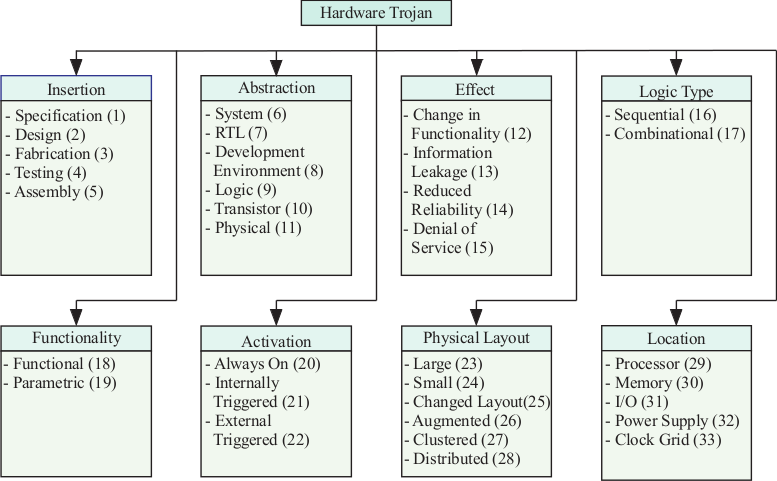
\includegraphics[width=0.7\linewidth]{../Thesis/Figures/HW_trojan}
%	\caption{The hardware trojan attribute taxonomy \cite{samerAttribute}.}
%	\label{fig:HW_trojan}
%\end{figure*}
%%%%%%%%%%%%%%%%%%%%%%%%%%
%\begin{enumerate}
%	\item The \textbf{insertion} (chip life-cycle) level comprises the attributes pertaining to the IC production stages.
%	\item The \textbf{abstraction} level corresponds to where in the IC abstraction the trojan is introduced.
%	\item The \textbf{properties} level comprises the behavior and physical characteristics of the trojan.
%	It contains the taxonomy categories \textit{effect}, \textit{logic type}, \textit{functionality}, \textit{activation} and \textit{layout}.
%	\item The \textbf{location} level corresponds to the location of the trojan in the IC.
%\end{enumerate}
%\begin{figure}[]
%	\centering
%	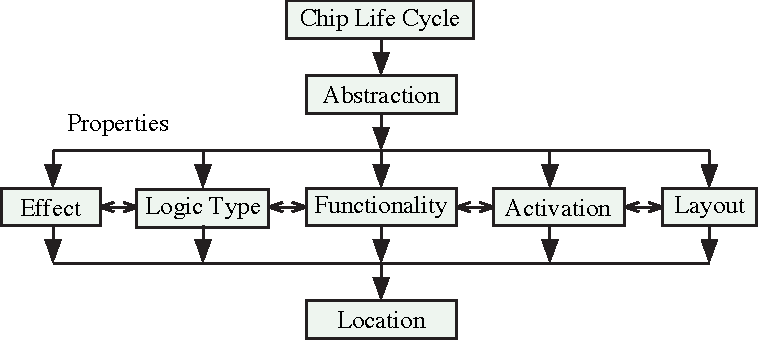
\includegraphics[width=0.99\linewidth]{../Thesis/Figures/trojan_life_cycle}
%	\caption{Hardware trojan life-cycle levels \cite{samerAttribute}.}
%	\label{fig:trojan_life_cycle}
%\end{figure}
%The properties level has the following categories.
%\begin{itemize}
%	\item The \textbf{effect} category describes the disruption or effect a trojan has on the system.
%	\item The \textbf{logic type} category describes the circuit logic that triggers the trojan, either combinational logic or sequential.
%	\item The \textbf{functionality} category differentiates between trojans which are functional or parametric.
%	\item The \textbf{activation} category differentiates between trojans which are always on or are triggered.
%	\item The \textbf{layout} category is based on the physical characteristics of the trojan.
%\end{itemize}
%The relationships between the trojan attributes shown in Fig.~\ref{fig:HW_trojan} can be described using a matrix $\mathbf{R}$~\cite{samerAttribute}.
%Entry $r(i,j)$ in $\mathbf{R}$ indicates whether or not attribute $i$ can lead to attribute $j$.
%For example, $r(2,3) = 1$ indicates that design (attribute 2) can lead to fabrication (attribute 3).
%This implies that if an IC can be compromised during the design phase (attribute 2), it may influence the fabrication phase (attribute 3).
%
%The matrix $\mathbf{R}$ is divided into sub matrices as follows
%\[
%\newcommand\scalemath[2]{\scalebox{#1}{\mbox{\ensuremath{\displaystyle #2}}}}
%\mathbf{R} =\left[
%\scalemath{1.1}{
%	\begin{array}{l*{3}{c}}
%	\mathbf{R_1} ~ & ~ \mathbf{R_{12}} ~ & ~ 0 ~  &  ~ 0   \\
%	0         & \mathbf{R_2}      &\mathbf{R_{23}}       & ~ 0 \\
%	0          & 0           & \mathbf{R_3}          & ~ \mathbf{R_{34}} \\
%	0          & 0           & 0                & ~ \mathbf{R_4} \\
%	\end{array}
%}
%\right]
%\label{R}
%\]
%where $\mathbf{R_1}$, $\mathbf{R_2}$, $\mathbf{R_3}$ and $\mathbf{R_4}$ indicate the attribute relationships within a category.
%For example, $\mathbf{R_1}$ is given by
%\[
%\newcommand\scalemath[2]{\scalebox{#1}{\mbox{\ensuremath{\displaystyle #2}}}}
%\mathbf{R_1} =\left[
%\scalemath{1.0}{
%	\begin{array}{l|*{11}{c}}
%	A & 1$~$ & 2$~$  & 3$~$ & 4$~$& 5$~$\\ \hline
%	1 & 0 & 1 & 0 & 0 & 0  \\
%	2 & 0 & 0 & 1 & 0 & 0  \\
%	3 & 0 & 0 & 0 & 1 & 0  \\
%	4 & 0 & 0 & 0 & 0 & 1  \\
%	5 & 0 & 0 & 0 & 0 & 0  \\
%	\end{array}
%}
%\right ]
%\label{R1}
%\]
%Submatrix $\mathbf{R_{12}}$ relates the attributes of the insertion category to the attributes of the abstraction category.
%An example of this submatrix is
%\[
%\newcommand\scalemath[2]{\scalebox{#1}{\mbox{\ensuremath{\displaystyle #2}}}}
%\mathbf{R_{12}} =\left[
%\scalemath{1.0}{
%	\begin{array}{l|*{11}{c}}
%	A & 6$~$  & 7$~$ & 8$~$ & 9$~$ & 10  & 11\\ \hline
%	1  & 1 & 0 & 0 & 0 & 0 & 0 \\
%	2  & 0 & 1 & 0 & 0 & 0 & 0 \\
%	3  & 0 & 0 & 0 & 0 & 0 & 1 \\
%	4  & 1 & 0 & 0 & 1 & 0 & 0 \\
%	5  & 1 & 0 & 0 & 0 & 0 & 0 \\
%	\end{array}
%}
%\right ]
%\label{R12}
%\]
%
%%%%%%%%%%%%%%%%%%%%%%%%%%%%%%%%
%\subsection{\acrlong{FPGAs}}
%An \acrfull{IC} belongs to one of two categories.
%An \acrfull{ASIC} or a \acrfull{FPGA}.
%An \acrshort{ASIC} is manufactured once and is immutable; its hardware is permanently printed into its silicon.
%\acrshort{FPGA}s are reconfigurable because they are comprised of an array of \acrfull{PLDs}.
%A \acrshort{PLD} is a component whose functionality is dependent on a set of configuration options; in other words, a user can define how it behaves.
%Each \acrshort{PLD} receives configuration instructions from the user that defines its functionality; these instructions are in the form of a binary message.
%In \Xilinx terminology a \acrshort{PLD} is referred to as a tile. 
%A single \acrshort{FPGA} can contain hundreds, or even thousands of tiles; a device is usually made up of over a hundred different types.
%Different types are used for different functions, such as \acrfull{IO}, Logic, Memory...etc.
%The set of messages sent to all of the tiles in the device from the user is referred to as the configuration \gls{Bitstream}.
%\acrshort{FPGA} users create designs using a programming language referred to as a \acrfull{HDL}.
%The design is then compiled and synthesized into the \gls{Bitstream} which is then downloaded or "configured" onto the device.
%\begin{figure}[h]
%	\centering
%	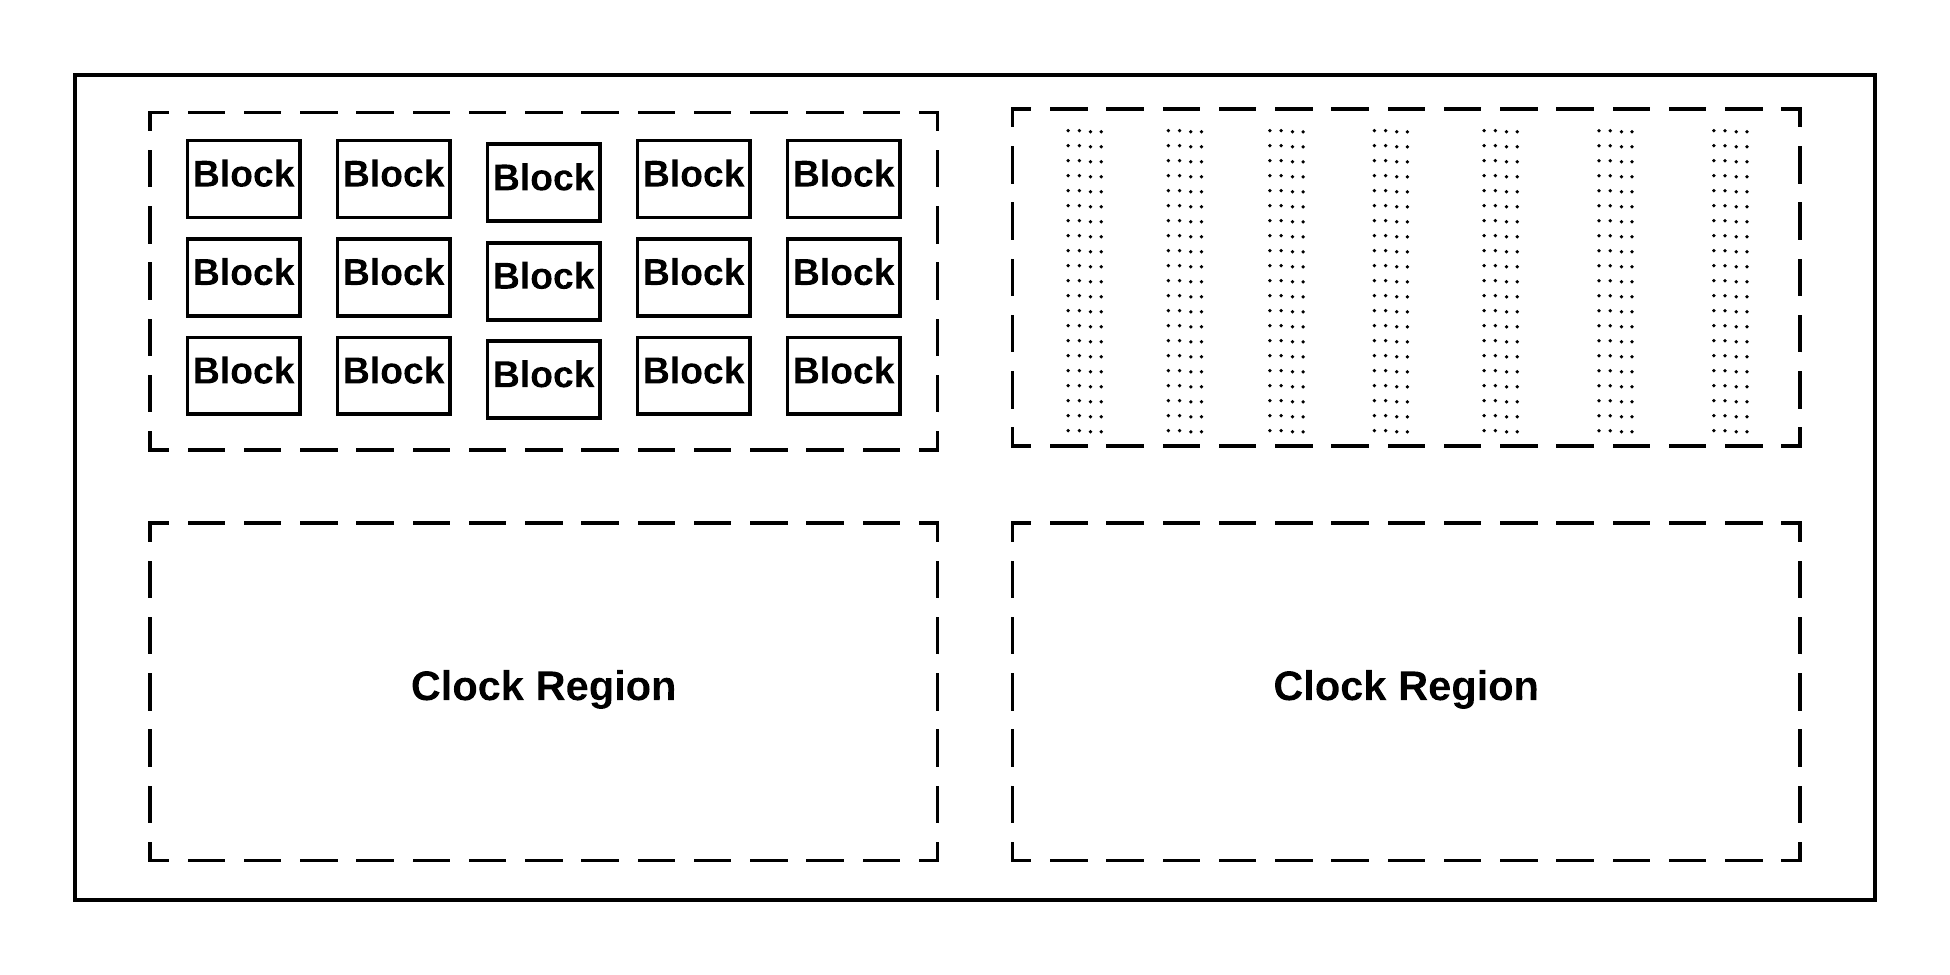
\includegraphics[width=1\linewidth]{../Thesis/Figures/FPGA}
%	\caption[Rudimentary Layout of a Virtex \acrshort{FPGA}]{Rudimentary Layout of a Virtex \acrshort{FPGA}}
%	\label{fig:FPGA}
%\end{figure}
%A \Xilinx \acrfull{FPGA} is comprised of a matrix of blocks referred to as the 'gate-array' and is shown in Figure~\ref{fig:FPGA}~\cite{xilnxDevManual}.
%A device can contain anywhere from a couple hundred to a few thousand blocks and are arranged into columns by type.
%Columns are separated into regions shown by the dashed lines in Figure~\ref{fig:FPGA}.
%These regions each use a separate clock mechanism and are referred to as 'Clock Regions'.
%
%The \Xilinx \gls{Bitstream} is a binary file composed of a series of 32-bit words organized into 'frames'.
%A frame is a string of single bits that span from the top to the bottom of a clock region of a device as seen in the top-right quadrant of Figure~\ref{fig:FPGA}.
%A frame affects every block in a column and multiple horizontally adjacent frames are required to configure an entire column.
%Each frame is uniquely identified by a 32-bit address and is the smallest addressable element.
%\begin{figure}[h]
%	\centering
%	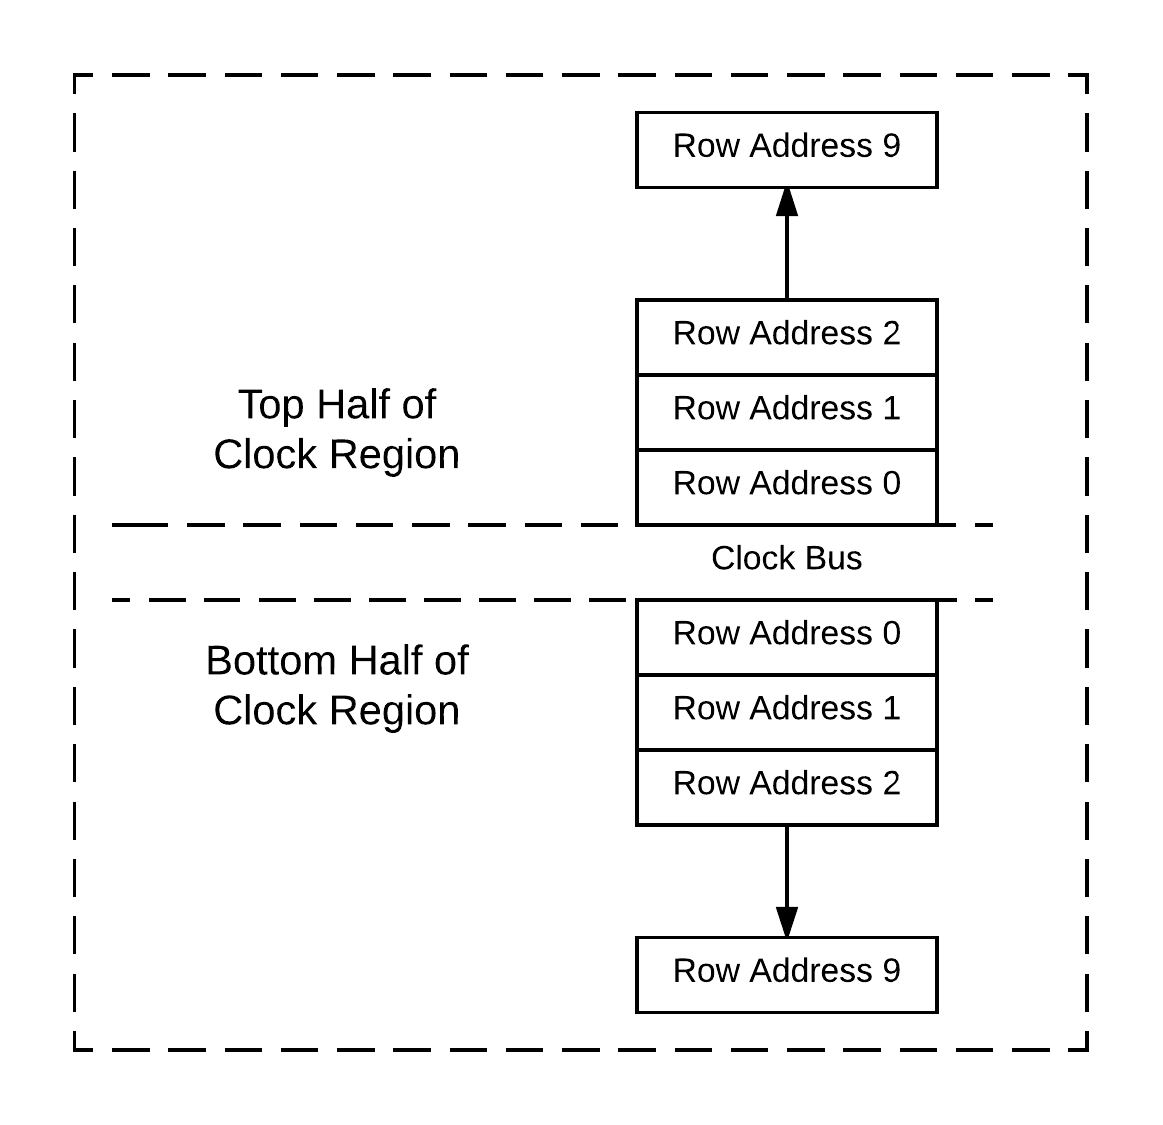
\includegraphics[width=.85\linewidth]{../Thesis/Figures/RowOrder}
%	\caption[Row Order of Virtex-5 Clock Region]{Row Order of Virtex-5 Clock Region}
%	\label{fig:RowOrder}
%\end{figure}
%Each clock region is given a row value in its address that increments away from the center of the device starting at 0. 
%%The frame address includes a Top indicator bit in position 20 that indicates whether the specified row is above or below the center of the device~\cite{virtex5ConfigGuide}.
%The major address specifies the column within the row.
%These addresses are numbered from left to right and begin at 0.
%The minor address indicates the frame number within a column. 
%Table~\ref{tbl:minorAddressNumbers} provides the number of frames per column type.
%\begin{table}[h!]
%	\centering
%	\caption{Number of Frames (minor addresses) per Column~\cite{virtex5ConfigGuide}}
%	\label{tbl:minorAddressNumbers}
%	\begin{tabular}{|c|c|}
%		\hline
%		Block             & Number Of Frames \\ \hline
%		CLB               & 36               \\ \hline
%		DSP               & 28               \\ \hline
%		\acrshort{BRAM}   & 30               \\ \hline
%		IOB               & 54               \\ \hline
%		Clock             & 4                \\ \hline
%	\end{tabular}
%\end{table}
%Frames are numbered from left to right, starting with 0. 
%A block may contain multiple tiles.
%In a \acrshort{CLB} column a block consists of an interconnect tile (also known as a \acrfull{SM}) and a \acrshort{CLB}.
%For each block frames numbered 0 to 25 access the interconnect tile for that column. 
%For all blocks, except the \acrshort{CLB} and the clock column, frames numbered 26 and 27 access the Interface for that column. 
%All other frames are specific to that block~\cite{virtex5ConfigGuide}.

%%%%%%%%%%%%%%%%%%%%%%%%%%%%%%%%%%%%%%%%%%%%%%%%%%%%%%%%%%%%%%%%%%%
\section{Methodology}
Figure~\ref{fig:Concept} provides a visual representation of the use-case assumed for the purposes of this work. 
With the exception of the fabrication process, all stages of production of an \acrshort{FPGA} implementation are assumed to have been done "in-house". 
Any trojan discovered is inserted in the fabrication phase; all other stages are trusted.  
The method of automated trojan detection described in this work would take place in the 'testing' phase of the life-cycle. 
\begin{figure}[h]
	\centering
	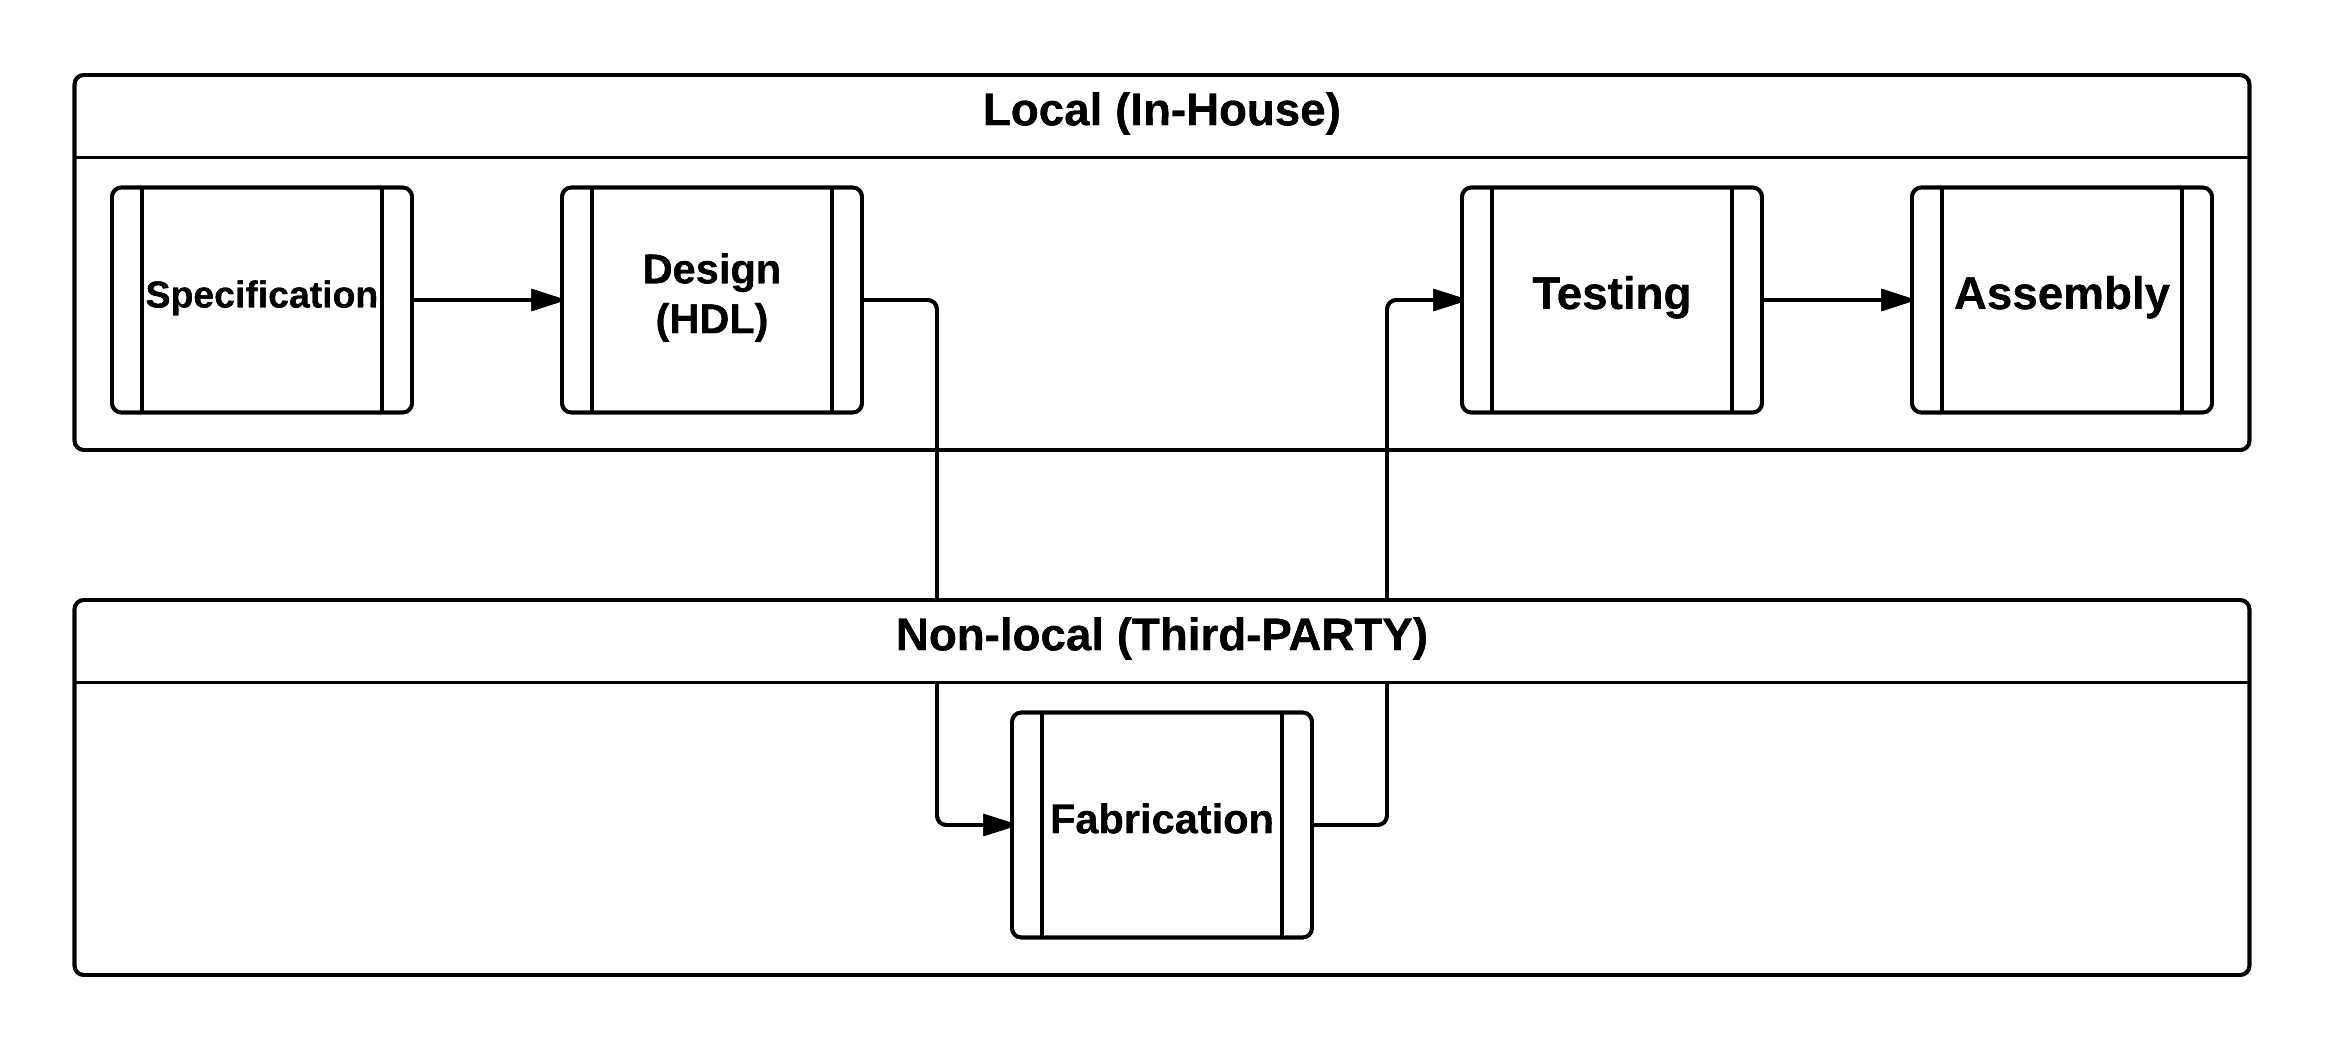
\includegraphics[width=1\linewidth]{../Thesis/Figures/Concept}
	\caption[FPGA Life-Cycle]{FPGA Life-Cycle}
	\label{fig:Concept}
\end{figure}
Figure~\ref{fig:methodologyOverview} shows an overview of the trojan detection methodology.
As mentioned, \acrshort{FPGA} designs are written in a \acrfull{HDL}.
\Xilinx provides a series of \acrfull{UI} and command line tools to process the \acrshort{HDL} known as the 'tool-chain'.
The tool chain generates a series of files that are used for a variety of purposes as shown in the 'Resultant Files' box in Figure~\ref{fig:methodologyOverview}.
The NGC file is a non-human readable semantic description of the design known as a netlist.
This file can be converted into a human-readable version known as \acrfull{XDL} which will be described in section~\ref{sec:XDL}.
The Bit file is the binary representation of the design to be implemented.
It is referred to as the \gls{Bitstream} or 'configuration' \gls{Bitstream} and is the final form that is loaded into the \acrshort{FPGA}.
\begin{figure}
	\centering
	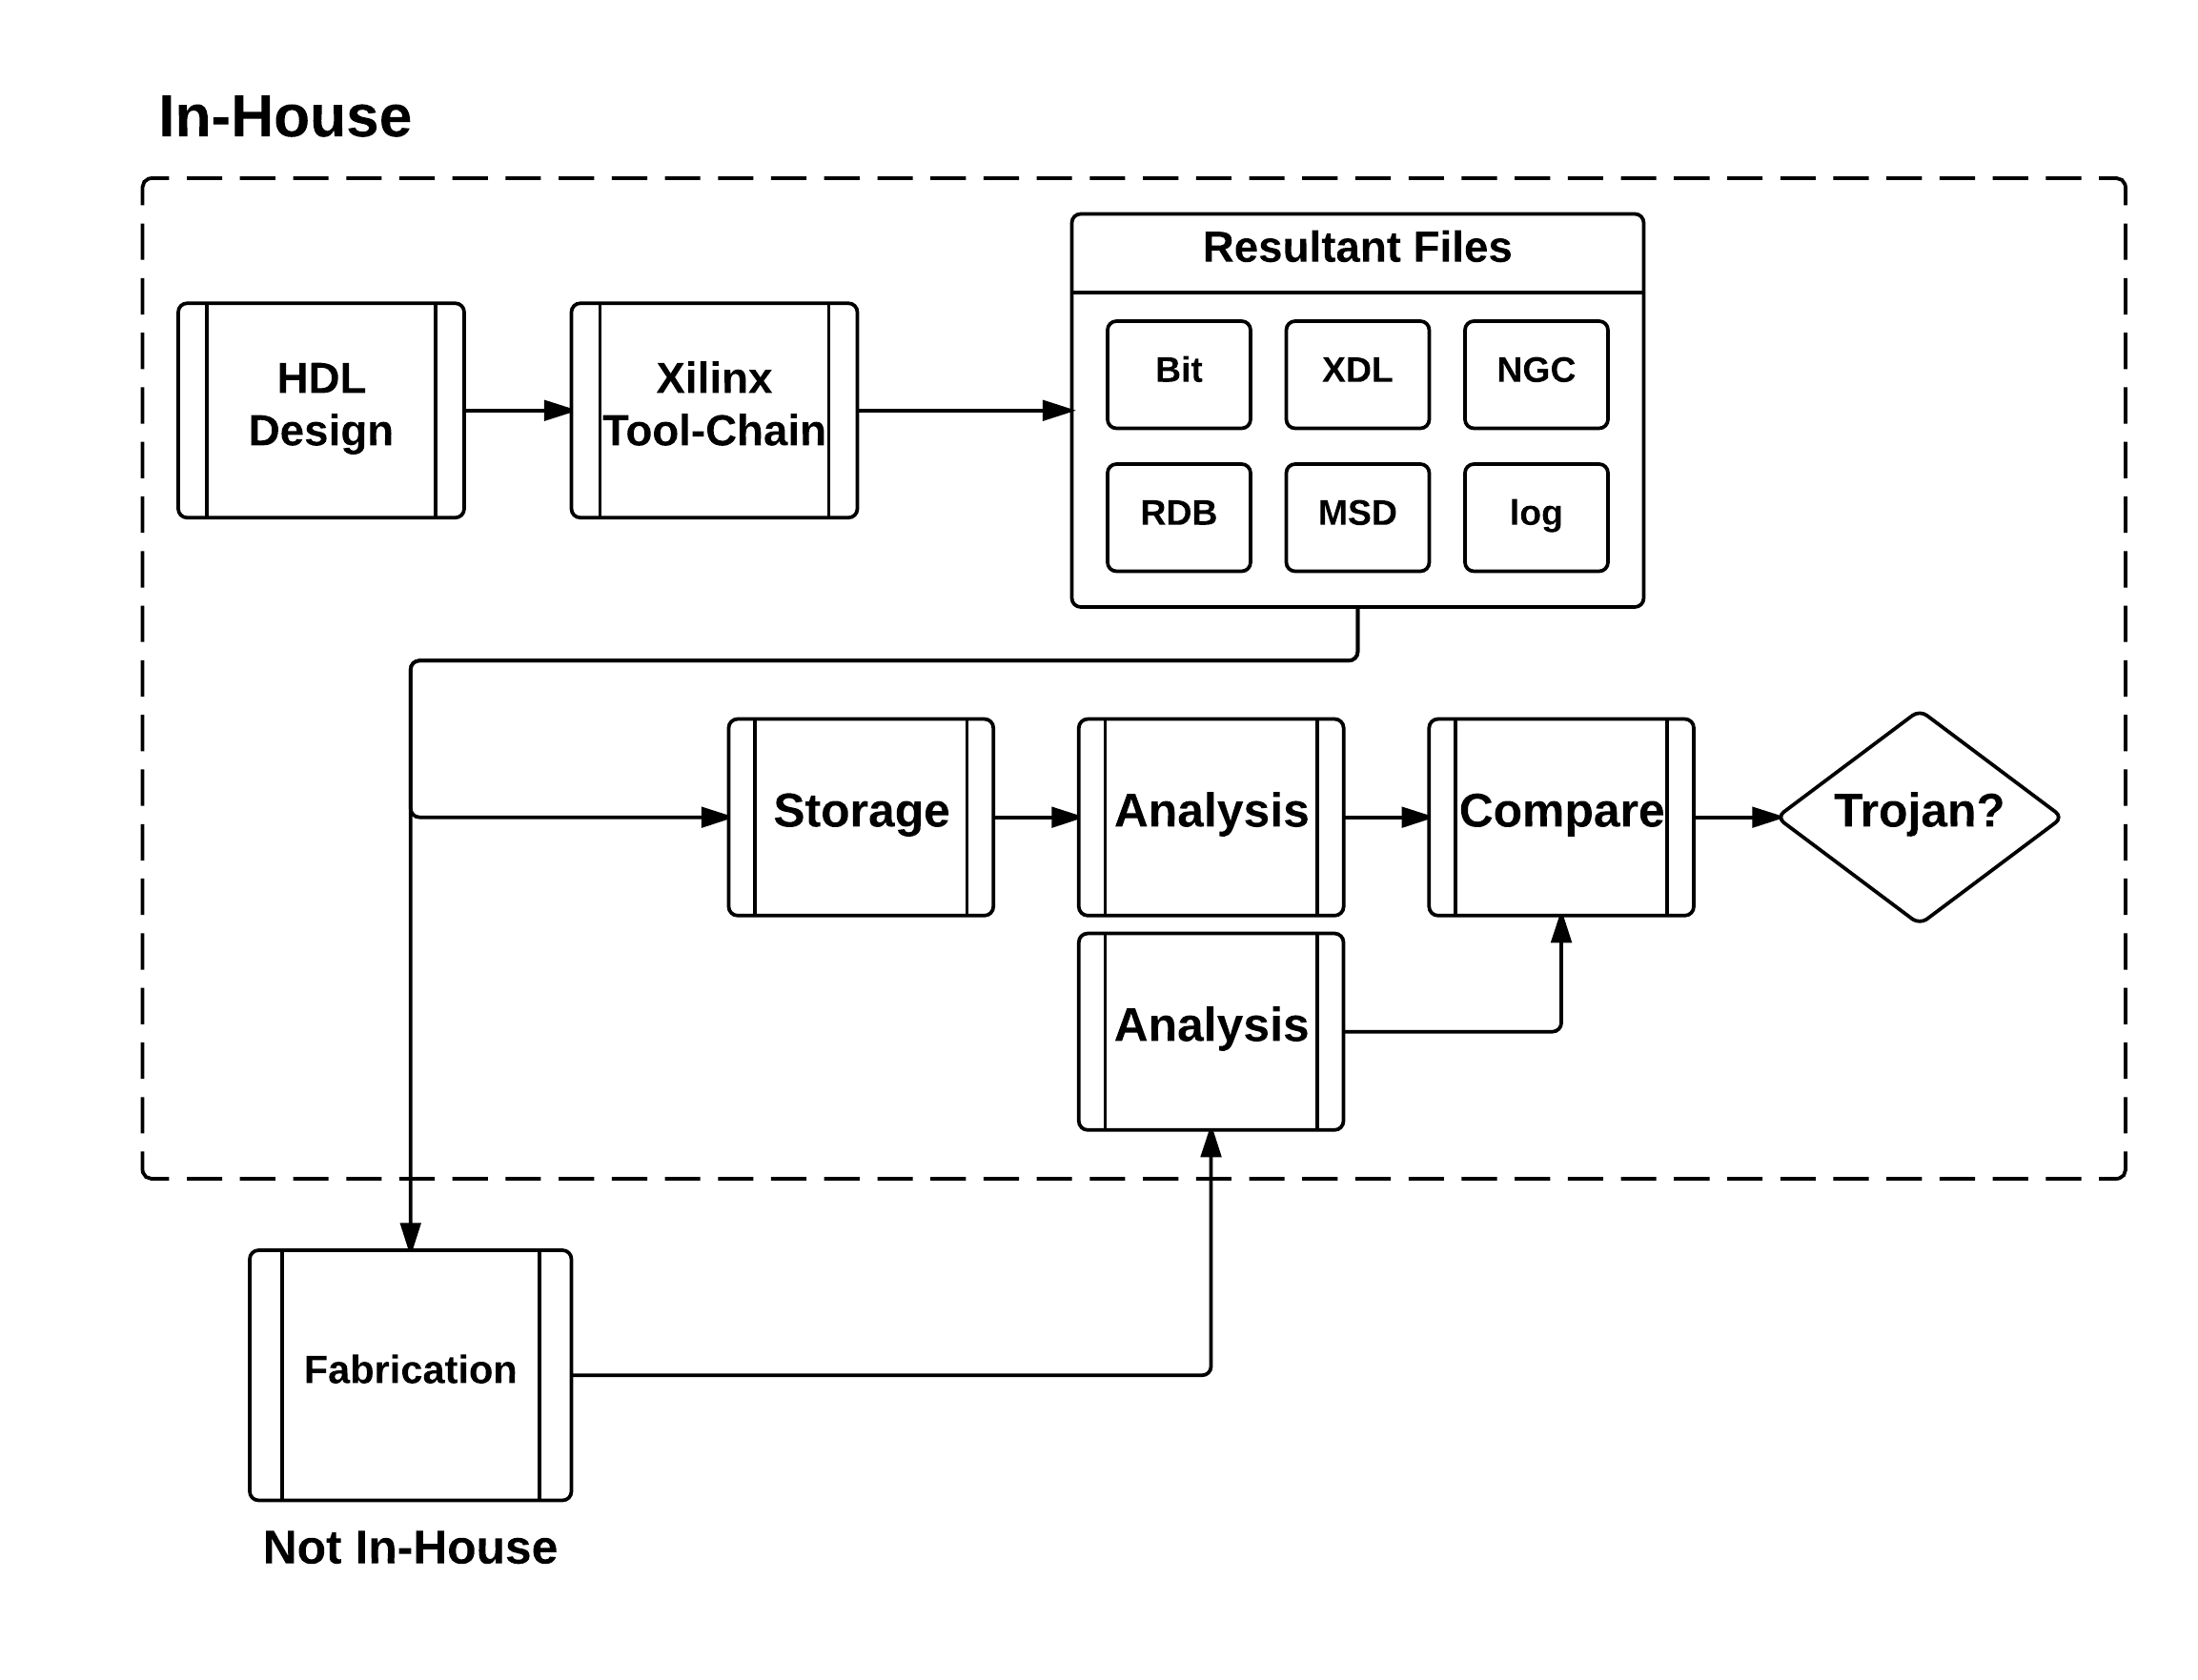
\includegraphics[width=1\linewidth]{../Thesis/Figures/methodologyOverview}
	\caption[Methodology Overview]{Methodology Overview}
	\label{fig:methodologyOverview}
\end{figure}
This Bit file is the primary file sent to the fabrication house where it will be implemented onto the batch of devices ordered.
The resultant files, produced 'in-house' are to be kept in secure storage while a copy is sent to be fabricated; these stored copies are referred to as \gls{golden} and assumed to be trojan-free.
Though it is known that the fabrication houses will often attempt to make optimizations on designs, this methodology requires that no such efforts be made.
When the completed batch of fabricated chips are returned the \gls{Bitstream} is extracted from a sample using the \Xilinx feature \gls{Readback}. 
That which is extracted is referred to as the \gls{target} \gls{Bitstream}.
The \gls{golden} and \gls{target} \gls{Bitstream}s are analyzed in conjunction to detect differences.
Any discovered differences are then attributed to the corresponding component in the architecture, described in section~\ref{sec:tileMapping}.
Finally, the resultant taxonomic description is returned to the user.

%%%%%%%%%%%%%%%%%%%%%%%%%%%%%%%
\subsection{The \acrshort{FPGA} \gls{Bitstream} Analysis} \label{sec:fpgaBitStream}
The \Xilinx \gls{Bitstream} is a binary file composed of a series of 32-bit words organized into 'frames'.
A frame is a string of single bits that span from the top to the bottom of a clock region of a device as seen in the top-right quadrant of Figure~\ref{fig:FPGA}.
A frame affects every block in a column and multiple horizontally adjacent frames are required to configure an entire column.
Each frame is uniquely identified by a 32-bit address and is the smallest addressable element.
The composition of the frame address is fairly consistent across the \Xilinx catalog however there are small differences between device families.
The following is the structure of the Virtex-5 family frame address scheme according to~\cite{virtex5ConfigGuide}.
The make-up of a frame address is shown in Table~\ref{tbl:frameAddress}.
\begin{table*}[t!]
	\centering
	\caption{Frame Address}
	\label{tbl:frameAddress}
	\resizebox{\textwidth}{!}{
		\begin{tabular}{|c|c|c|c|c|c|c|c|c|c|c|c|c|c|c|c|c|c|c|c|c|c|c|c|c|c|c|c|c|c|c|c|}
			\hline
			\multicolumn{8}{|c|}{Unused} & \multicolumn{3}{c|}{BA} & T & \multicolumn{5}{c|}{Row Address} & \multicolumn{8}{c|}{Major Address} & \multicolumn{7}{c|}{Minor Address} \\ \hline
			31 & 30 & 29 & 28 & 27 & 26 & 25 & 24 & 23 & 22 & 21 & 20 & 19 & 18 & 17 & 16 & 15 & 14 & 13 & 12 & 11 & 10 & 9 & 8 & 7 & 6 & 5 & 4 & 3 & 2 & 1 & 0 \\ \hline
			0 & 0 & 0 & 0 & 0 & x & x & x & x & x & x & x & x & x & x & x & x & x & x & x & x & x & x & 0 & 0 & 0 & 0 & 0 & 0 & 0 & 0 & 0 \\ \hline
		\end{tabular}		
	}
\end{table*}

The \acrfull{BA} identifies the block type.
\begin{itemize}
	\item BA 0: Logic type.
	\item BA 1: \acrfull{BRAM}.
	\item BA 2: \acrshort{BRAM} Interconnect.
	\item BA 3: \acrshort{BRAM} non-configuration frame.
\end{itemize}
The logic block contains the columns which provides the primary configuration for the device (\acrshort{CLBs}, \acrshort{IOBs}... etc).
The \acrshort{BRAM} columns initialize the memory for the device while the \acrshort{BRAM} Interconnect columns configure how the logic of the design interacts with the \acrshort{BRAM}.

%In the case of the Virtex-5 family each clock region is composed of twenty blocks in a column separated by a horizontal clock bus as shown in Figure~\ref{fig:RowOrder}.
\begin{figure}[h]
	\centering
	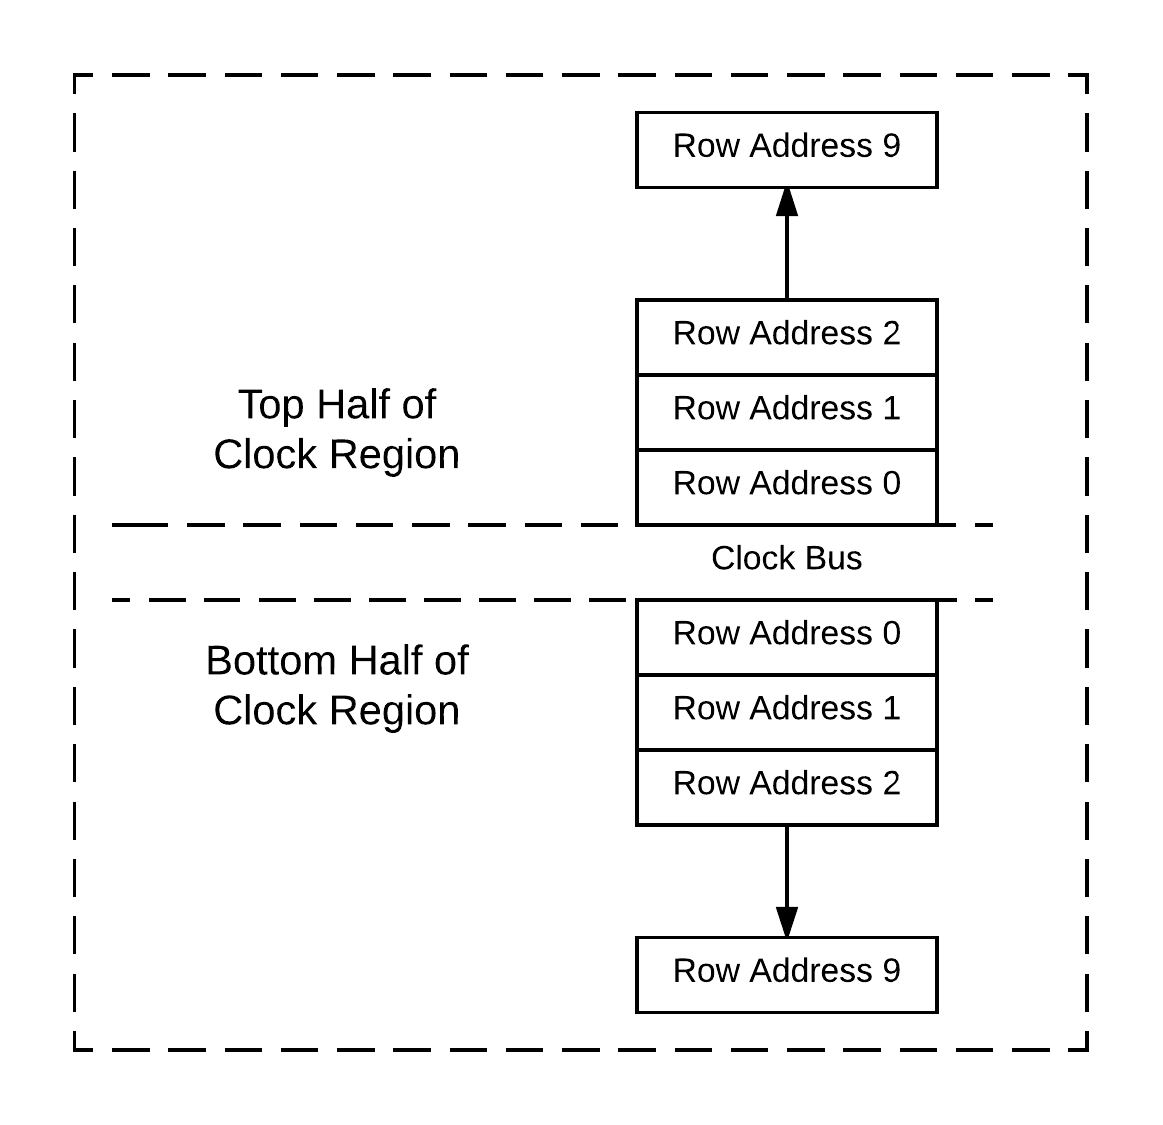
\includegraphics[width=.7\linewidth]{../Thesis/Figures/RowOrder}
	\caption[Row Order of Virtex-5 Clock Region]{Row Order of Virtex-5 Clock Region}
	\label{fig:RowOrder}
\end{figure}
Each clock region is given a row value in its address that increments away from the center of the device starting at 0. 
The frame address includes a Top indicator bit in position 20 that indicates whether the specified row is above or below the center of the device~\cite{virtex5ConfigGuide}.
The major address specifies the column within the row.
These addresses are numbered from left to right and begin at 0.
The minor address indicates the frame number within a column. 
Table~\ref{tbl:minorAddressNumbers} provides the number of frames per column type.
\begin{table}[h!]
	\centering
	\caption{Number of Frames (minor addresses) per Column~\cite{virtex5ConfigGuide}}
	\label{tbl:minorAddressNumbers}
	\begin{tabular}{|c|c|}
		\hline
		Block             & Number Of Frames \\ \hline
		CLB               & 36               \\ \hline
		DSP               & 28               \\ \hline
		\acrshort{BRAM}   & 30               \\ \hline
		IOB               & 54               \\ \hline
		Clock             & 4                \\ \hline
	\end{tabular}
\end{table}
A block may contain multiple tiles.
In a \acrshort{CLB} column a block consists of an interconnect tile, also known as a \acrfull{SM} and a \acrshort{CLB}.
Frames are numbered from left to right, starting with 0. 
For each block, except in a clock column, frames numbered 0 to 25 access the interconnect tile for that column. 
For all blocks, except the \acrshort{CLB} and the clock column, frames numbered 26 and 27 access the Interface for that column. 
All other frames are specific to that block~\cite{virtex5ConfigGuide}.
To further understand how frames configure tiles a mapping must be made between each frame and the corresponding tile.
This is described in section~\ref{sec:tileMapping}.

%%%%%%%%%%%%%%%%%%%%%%%%%%%%%%%
\subsection{Component Mapping} \label{sec:tileMapping}
The \NameNoPeriod employs a method referred to as Component Mapping to create a mapping between each word in a configuration frame and the component on the device that it configures.
This information is not publicly released by \Xilinx as a means of providing security through obscurity.

\subsubsection{Frame to Column Mapping}
The configuration \gls{Bitstream} is stored in an external memory device as described in section~\ref{sec:architectureAndConfig}.
When powered-on the \gls{Bitstream} is transmitted in frame address order to populate the dynamic memory in the tiles of the gate-array.
The frame addressing scheme describes where in the gate-array the frame is destined fairly directly.
Frames with a \acrshort{BA} value of 1 are clearly destined to configure the \acrshort{BRAM} and do not need further analysis for the purposes of this method.
Frames with a \acrshort{BA} value of 0 or 2 must be mapped more finitely.
The row address specifies which row of clock-regions the frame is destined.
Figure~\ref{fig:FPGA} shows four clock regions organized into two rows. 

As an example the Virtex-5 240T has 12 rows; its row address spans from 0-5 and the Top bit in the address indicates whether it is in the top or bottom half of the device in accordance with Figure~\ref{fig:RowOrder}.
Once the correct clock region is discerned the major address is used to determine which column the frame configures.
The major address begins at 0 on the left and counts up towards the number of columns in the row.
Finally, the minor address is used to determine which sub-column has been modified according to Table~\ref{tbl:frameAddress}.
\subsubsection{Word to Block Mapping}
In the case of Virtex-5 devices a frame is composed of 41 words that can be thought of as a vertical stack that aligns with a column.
As described in section~\ref{sec:fpgaBitStream} a row consists of a stack of basic blocks; there are 20 \acrshort{CLB} blocks per column, 40 \acrshort{IOB}s, 4 \acrshort{BRAM}...etc for Virtex-5 devices.
\begin{figure}[h]
	\centering
	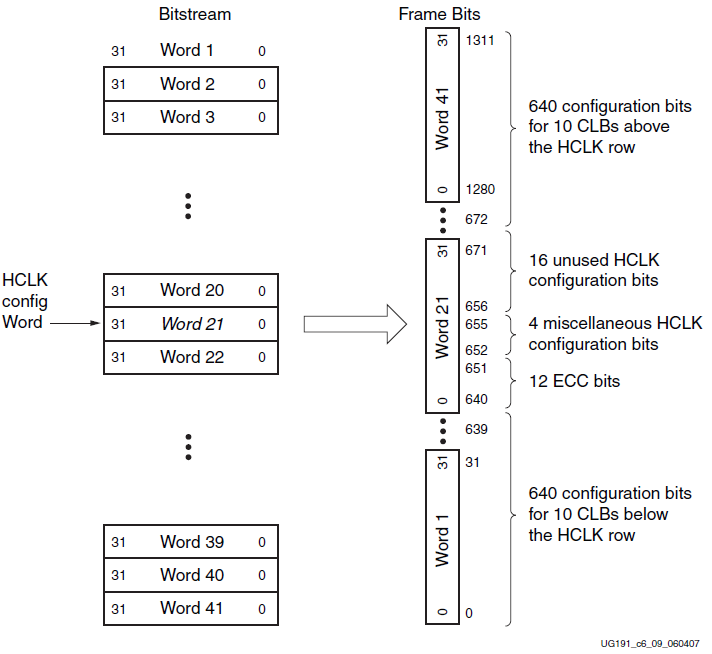
\includegraphics[width=0.9\linewidth]{../Thesis/Figures/frameTileMap}
	\caption[Configuration Words in the Bitstream~\cite{virtex5ConfigGuide}]{Configuration Words in the Bitstream~\cite{virtex5ConfigGuide}}
	\label{fig:frameTileMap}
\end{figure}
As can be seen in Figure~\ref{fig:frameTileMap} the central word in a frame configures the horizontally running clock bus.
The remaining words are used to configure the blocks in the column.
The purpose of the central word in the column is known to be mapped to the clock bus.
For the purposes of the following computations it is considered removed from the frame.
From this, equation~\ref{eqn:numWordsPerBlock} can be deduced which is used to compute the number of 32-bit words that span each block.
\begin{equation} \label{eqn:numWordsPerBlock}
n = (W - C) + B
\end{equation}
\ConditionSize
where:
\begin{conditions}
	n     &  Number of Words per Block \\
	W     &  Number of 32-bit words per frame \\   
	C     &  Number of clock words per frame \\
	B     &  Number of blocks per column
\end{conditions}
\normalsize
As shown in Figure~\ref{fig:frameTileMap} words are addressed from the 'top' of a device down.
Equation~\ref{eqn:getTileNumber} can be used to map a particular word in a frame to a block on the device.
\begin{equation} \label{eqn:getTileNumber}
i = B - \floor*{\frac{w}{n}}
\end{equation}
\ConditionSize
where:
\begin{conditions}
	i     &  Word Number in frame\\
	B     &  Number of blocks per column \\
	w     &  Word number \\
	n     &  Number of Words per Block 
\end{conditions}
\normalsize
With equations~\ref{eqn:numWordsPerBlock} and~\ref{eqn:getTileNumber} it is now possible attribute any modifications in the \gls{Bitstream} to its corresponding block.

\subsection{Determining Trojan Attributes} \label{sec:trojanAttributes}
The complexity of \acrlong{IC} designs and their corresponding trojans requires a more human-friendly scope.
The taxonomy in~\cite{samerAttribute} provides a series of thirty-three attributes which a trojan may or may not posses.
Though it is desirable to be able to observe and directly extract the attributes a trojan possesses it is not always possible. 
In~\cite{samerAttribute} a matrix, $\mathbf{R}$, is provided which describes the relationships between each of the thirty-three attributes in the taxonomy.
When it is not possible to directly determine the presence of certain attributes, this relation matrix is used to infer their existence.
The analysis stage of the automated trojan detection technique provided by this work begins by extracting those attributes that are directly observable then using matrix $\mathbf{R}$ to infer the existence of the remainder. 
\subsubsection{Observed Location Attributes}
The presence of attributes in the \textit{Location} category are directly observable from the results of the component mapping method described in section~\ref{sec:tileMapping}.
\Xilinx tiles conform to purpose-specific groups or block types which were discussed in section~\ref{sec:fpgaBitStream}.
These block types contain sub-types that perform actions which pertain to the \textit{Location}, category. 
\begin{enumerate}
	\item The \textbf{Processor} attribute pertains to the core functionality of the design logic. It can be awarded for presence of a modified \acrshort{CLB} tile or Interconnect tile.
	\item The \textbf{Memory} attribute can be awarded for the presence of modified \acrshort{BRAM} components.
	\item The \textbf{\acrshort{IO}} attribute can be awarded for presence of modified \acrshort{IOB} tiles.
	\item The \textbf{Power Supply} attribute can be awarded for the presence of modified interface or configuration tiles.
	\item The \textbf{Clock Grid} attribute can be awarded for modified clock tiles.
\end{enumerate}
\subsubsection{Scatter Score Method} \label{sec:scatterScore}
The gate-array configuration of components in \Xilinx \acrshort{FPGA}s allows for an analytical method of determining attributes in the \textit{Physical Layout} category.
The "Scatter Score" method uses the grid coordinates of components to derive a numerical score rating for the size, position, and augmentation of configured tiles.
Tiles are assigned global coordinates that represent their horizontal and vertical positions within the gate array denoted $x$ and $y$ respectively. 
These values can then be used to strongly infer the presence of \textit{Physical Location} attributes.

The golden chip is first analyzed.
The set of all tiles which are configured in the golden design is found and a series of numerical descriptors are computed.
\begin{equation} \label{eqn:numConfiguredTiles}
n = \sum_{x = 0}^{X}\sum_{y = 0}^{Y}T_{xy}
\end{equation}
\ConditionSize
where:
\begin{conditions}
	n     &  Number of all \textbf{configured} tiles \\
	X     &  The column width of the gate-array \\   
	Y     &  The number of rows of the gate-array \\
	T     &  A configured tile
\end{conditions}
\normalsize

\noindent\begin{minipage}{.5\linewidth}
	\begin{equation} \label{eqn:xAverage}
	a_x = \frac{1}{n}\sum_{x=0}^{n}T_x
	\end{equation}
\end{minipage}%
\begin{minipage}{.5\linewidth}
	\begin{equation} \label{eqn:yAverage}
	a_y = \frac{1}{n}\sum_{y=0}^{n}T_y
	\end{equation}
\end{minipage}
\\
\noindent\begin{minipage}{.5\linewidth}
	\begin{equation} \label{eqn:stdDevX}
	\sigma_x = \sqrt{\frac{1}{n}\sum_{x = 0}^{X}(x_i - a_x)^2)}
	\end{equation}
\end{minipage}%
\begin{minipage}{.5\linewidth}
	\begin{equation} \label{eqn:stdDevY}
	\sigma_y = \sqrt{\frac{1}{n}\sum_{y = 0}^{Y}(y_i - a_y)^2)}
	\end{equation}
\end{minipage}

\ConditionSize
where:
\begin{conditions}
	$$a_x$$     &  The average x coordinate of configured tiles \\   
	$$a_y$$     &  The average y coordinate of configured tiles \\
	$$T_x$$     &  The x coordinate of a configured tile \\
	$$T_y$$	    &  The y coordinate of a configured tile \\
	$$\sigma_x$$ & The standard deviation of the x coordinate of configured tiles \\
	$$\sigma_y$$ & The standard deviation of the y coordinate of configured tiles
\end{conditions}
\normalsize
Equations~\ref{eqn:xAverage} and~\ref{eqn:yAverage} are used to create a rating known as the \gls{positionMedian} in Equation~\ref{eqn:positionMedian}.
The \gls{positionMedian} value provides a simple descriptor for where in the gate array the design is centralized.
The \gls{scatterScore} in Equation~\ref{eqn:scatterScore} describes how spread out or, \textit{clustered} the design is.

\noindent\begin{minipage}{.5\linewidth}
	\begin{equation} \label{eqn:positionMedian}
	M_{xy} = (a_x,~a_y)
	\end{equation}
\end{minipage}%
\begin{minipage}{.5\linewidth}
	\begin{equation} \label{eqn:scatterScore}
	S_{xy} = (\sigma_x,~\sigma_y)
	\end{equation}
\end{minipage}
\ConditionSize

where:
\begin{conditions}
	$$M_{xy}$$     &  The \gls{positionMedian} \\   
	$$S_{xy}$$     &  The \gls{scatterScore}
\end{conditions}
\normalsize

The results of the component mapping method described in section~\ref{fig:frameTileMap} are used to generate the set of all tiles reconfigured by the trojan.
The set of reconfigured tiles can be said to contain three subsets: the subset of tiles activated by the trojan, those deactivated and those modified. 
The results of the golden design analysis, the subsets, and the numeric descriptors can be used to discern which of the \textit{Physical Location} attributes the trojan possesses. 
The \textit{Physical Location} category contains six attributes.
These six can be considered three pairs; a trojan exhibits one attribute from each pair. 
\begin{enumerate}
	\item \textbf{Large or Small} (attributes 23 or 24): According to~\cite{samerAttribute}, small trojans are defined as those that are nearly impossible to detect via power consumption. From this it can be said that 'small' trojans occupy minimal resources. Trojans where the number of reconfigured tiles is less than 5\% of the number of tiles in the golden design are considered small. Other wise they are attributed as large.
	\item \textbf{Changed Layout or Augmented} (attributes 25 or 26): A 'changed layout' trojan is such that only tiles that are configured by the golden design are reconfigured. An augmented trojan is where additional layout is added. The presence of 'activated' or 'deactivated' tiles indicates an augmented trojan. 
	\item \textbf{Clustered or Distributed} (attributes 27 or 28): The trojan is considered to be clustered when the standard deviation of the reconfigured tile positions is less than 15\%; distributed otherwise.
\end{enumerate}
\subsubsection{Insertion and Abstraction Attributes}
The linear nature of the manufacturing life-cycle implies a propagation of effects.
For the purposes of this method it is assumed that the only non-trustworthy stage in the life-cycle is fabrication.
In other words, the trojan was inserted in the third-party fabrication stage.
Due to the propagating nature of the life-cycle the effects of the modifications made in the fabrication stage (attribute 3) are felt in the testing (attribute 4) and assembly (attribute 5) stages.
Hence, it can be said that this trojan possesses insertion category attributes 3, 4 and 5.
\acrshort{FPGA} designs are made with a \acrshort{HDL}.
These languages dictate component arrangement in the \acrfull{RTL} abstraction level.
Hence it can be said that trojans occurring in \acrshort{FPGAs} take place in the System (attribute 6) and \acrshort{RTL} (attribute 7).
  
\subsubsection{Relation Matrix Use} \label{sec:matrixUse}
Attributes which are not directly observable can be inferred using a systematic method of analyzing the rows and columns of the relation matrix presented in~\cite{samerAttribute}.
The \NameNoPeriod takes the attributes it is able to directly observe and uses them as input to this process.
A thorough description of this method is given in~\cite{samerDissertation} and~\cite{meCategorization}.
\section{\Name}
\section{Results}
To demonstrate its potential, it has been tested using a series of benchmarks.
These benchmarks are included in the \NameNoPeriod application package as an example for users.
\subsection{Priority Decoder} \label{sec:priorityDecoder}
The \NameNoPeriod was first tested using a small 'Priority Decoder' circuit presented by F. Brglez and H. Fujiwara
in~~\cite{iscas85}.
The provided verilog code for the decoder benchmark was synthesized on a Virtex-5 XC5VLX155 and the generated \gls{Bitstream} and \acrshort{XDL} files were acquired.
The priority decoder \gls{Bitstream} file was fed to both the \gls{golden} and \gls{target} inputs to the \Name.
Feeding the same \gls{Bitstream} file to both inputs replicates the occurrence where the third-party fabrication house made no modifications; the \gls{Bitstream} extracted from the \gls{target} device is exactly the same as the \gls{golden}.
It is expected that the \NameNoPeriod returns a result indicating that there is no trojan present.
The \NameNoPeriod successfully analyzed the \gls{Bitstream}s and determined that there was no trojan present, as expected.

\subsection{User Authentication Circuit} \label{sec:userAuthentication}
Consider a circuit designed to compute a function $F(x)$ for a system to authenticate user-password pairs $x$ and $F(x)$.
The system performs the arithmetic operation $F(x) = x^2$ to validate users.
The customer wishes to provide access to ten users labeled $I_0$ to $I_9$.
To identify all ten users, four input bits are required, $x_1$ to $x_4$.
The largest function output is $81$ meaning seven bits are required for output, $Z_1$ to $Z_7$, as illustrated in Fig.~\ref{fig:userAuthenticationCircuit}.
A trojan can be inserted into this circuit as shown in Fig.~\ref{fig:userAuthenticationCircuitTrojan} (called a backdoor trojan).
\begin{figure}[h]
	\centering
	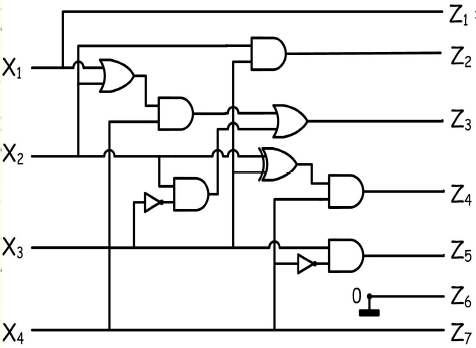
\includegraphics[width=0.7\linewidth]{../Thesis/Figures/circuit1}
	\caption{A Simple User Authentication Circuit}
	\label{fig:userAuthenticationCircuit}
\end{figure}
\begin{figure}[h]
	\centering
	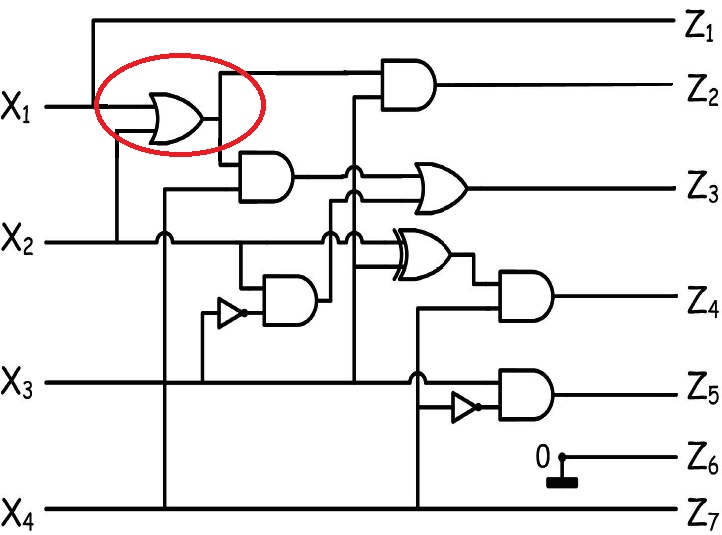
\includegraphics[width=0.7\linewidth]{../Thesis/Figures/circuit2}
	\caption{The Back-door Trojan}
	\label{fig:userAuthenticationCircuitTrojan}
\end{figure}
\begin{table}[h]
	\centering
	\caption{Outputs of the Circuits in Figs.~\ref{fig:userAuthenticationCircuit} and \ref{fig:userAuthenticationCircuitTrojan}~\cite{samerAttribute}}
	\label{tbl:trojanOutputs}
	\begin{tabular}{|c|c|c|c|c|}
		\hline
		& User Id & Input & Circuit A & Circuit B \\ \hline
		\multirow{5}{*}{\rotatebox[origin=c]{90}{Inputs}} & $I_0$ & 0 & 0 & 0 \\ \cline{2-5} 
		& $I_1$ & 1 & 1 & 1 \\ \cline{2-5} 
		& $I_2$ & 2 & 4 & 4 \\ \cline{2-5} 
		& : & : & : & : \\ \cline{2-5} 
		& $I_9$ & 9 & 81 & 81 \\ \hline
		\multirow{3}{*}{\rotatebox[origin=c]{90}{DC}} & $I_{10}$ & 10 & 68 & 100 \\ \cline{2-5} 
		& $I_{11}$ & 11 & 89 & 121 \\ \cline{2-5} 
		& : & : & : & : \\ \hline
	\end{tabular}
\end{table}
The outputs of the original and infected circuits are compared in Table~\ref{tbl:trojanOutputs}.
A simple test will show that the circuit outputs the desired $F(x) = x^2$ for each of the users.
However, upon closer inspection it is noted that the inputs corresponding to $x = 10$ to $x = 15$ are not used; there are no clients occupying those identifications.
These unused inputs are referred to as 'dont-cares' (DC), meaning that it is not important to the function of the circuit what their corresponding output is.
Don't-care cases are a typical vulnerability which can be exploited by an attacker.

The circuits shown in Figures~\ref{fig:userAuthenticationCircuit} and~\ref{fig:userAuthenticationCircuitTrojan} were implemented and synthesized on a Virtex-5 240T  (XC5VSX240T).
The resultant \gls{Bitstream}s were input to the \NameNoPeriod and the system output the attributes:
\begin{itemize}
	\item Attribute 3: Fabrication
	\item Attribute 4: Testing
	\item Attribute 5: Assembly
	\item Attribute 6: System
	\item Attribute 7: RTL
	\item Attribute 12: Change in Functionality
	\item Attribute 17: Combinational
	\item Attribute 18: Functional
	\item Attribute 20: Always On
	\item Attribute 24: Small
	\item Attribute 26: Augmented
	\item Attribute 27: Clustered
	\item Attribute 29: Processor
\end{itemize}
As expected the results state that the trojan was inserted in the Fabrication phase (3); it is the earliest stage in the 'insertion' phase produced indicating it as the source.
The effects of this modification propagate to the Testing (4) and Assembly (5) phases as expected.
The modifications reach both the System (6) and \acrfull{RTL} (7) abstraction levels.
Since the modifications were made using the schematic designer provided by \Xilinx which works in the \acrshort{RTL} level, these results are as expected.
The results indicate that the trojan Changes Functionality (12). 
This agrees with the modification to the values listed in Table~\ref{tbl:trojanOutputs}.
The trojan does not take affect over multiple clock cycles; this indicates it is composed of only Combinational (17) circuitry which is reflected in the results.
The trojan did not modify power levels or operation configurations, only design configurations.
This indicates that the trojan can be described as Functional (18), not Parametric (19); this agrees with the results.
Since the modification made a permanent alteration to the internal wiring of the circuit it can be said to be Always On (20).
The modified values for input $x=10$ or $x=11$ are always available and not activated.
This is consistent with the returned results.
The trojan changed only minor routing configurations in the circuit designs, this required the alteration of only a few tiles.
The new route required the activation of tiles which were not active in the \gls{golden} design; further, all of the modified tiles are nearby those in the \gls{golden} design. 
With these observations it can be said that this trojan exhibits Physical Layout attributes Small (24), Augmented (26) and Clustered (28). 
All of the expected Physical Layout attributes were correctly determined by the Scatter Score method of section~\ref{sec:scatterScore}.
Finally, all of the tiles modified by the trojan belong to major block type 0: Logic Type.
These tiles only affect the internal processing of the circuit.
No \acrshort{IOB}, Clock or \acrshort{BRAM} tiles were modified.
This is reflected by the fact that only Location attribute, Processor (29), was returned by the analysis.
The results observed by the experiment conformed with the experiments expectations demonstrating the accuracy of the method.
The entire analysis takes less than a minute to perform.

\subsection{AES-T100} \label{sec:aesT100}
In 2013 H. Salmani, M. Tehranipoor and R. Karri published a discussion on the design and development of \acrshort{FPGA} trojan benchmarks.
They collaboratively developed a series of verilog, VHDL and virtual machines that demonstrated effective creation of testable benchmarks.
They took the benchmarks they created and published them on a website they created called \textit{Trust-Hub}.
To demonstrate the efficacy of the \NameNoPeriod a benchmark named 'AES-T100' was chosen. 
From the description it is reasonable to expect certain results from the \Name.
The supporting documentation claims that the trojan 'leaks the secret key'.
From this we should expect our results to contain Effect attribute Information Leakage (13).
Information being leaked from a device will need a means to be transmitted to the attacker.
Location attribute \acrshort{IO} (31) may be observed.
It then states that it leaks 'single bits over many clock cycles'. 
This suggests that the trojan exhibits some form of Sequential Logic (16).
This may or may not require modification to clock tiles; Location attribute Clock Grid (33) may be observed. 
It then states that the PRNG is initialized to a predefined value; initialization requires the value be stored in memory. 
Location attribute Memory (30) should be expected.
The trojan then uses a 'power side-channel' as a communication channel.
This will require modification to power tiles; Location attribute Power Supply (32) should be expected.

The source code for the \gls{golden} and \gls{target} designs were downloaded from \textit{trust-hub.org} and synthesized on a Virtex-5 240T  (XC5VSX240T).
The resultant \gls{Bitstream}s were analyzed and the \NameNoPeriod output the following attributes which correlate well to the description in the documentation:
\begin{itemize}
	\item Attribute 3: Fabrication
	\item Attribute 4: Testing
	\item Attribute 5: Assembly
	\item Attribute 6: System
	\item Attribute 7: RTL
	\item Attribute 13: Information Leakage
	\item Attribute 16: Sequential
	\item Attribute 18: Functional
	\item Attribute 20: Always On
	\item Attribute 24: Large
	\item Attribute 26: Augmented
	\item Attribute 27: Distributed
	\item Attribute 29: Processor
	\item Attribute 30: Memory
	\item Attribute 31: \acrshort{IO}
	\item Attribute 32: Power Supply
	\item Attribute 33: Clock Grid
\end{itemize}
\section{Conclusion}
Configuration \gls{Bitstream}s are enormous strings of binary data.
To the human reader this information means nothing.
To an \acrshort{FPGA}, however, this data is everything.
Every conceivable design, and every possible trojan is contained within the \gls{Bitstream}.
Yet, due to the shear volume of information within it and the lack of details on its format it has not previously been a common subject of study.
With its success, \acrlong{IC} manufacturers that use \acrshort{FPGA}s will have an additional tool to ensure that their products operate as expected.
Using the \NameNoPeriod takes only a few button clicks on the \acrlong{UI}.
Its simple construction does not require any additional software or complicated install procedures and it can be used on any major operating system.
Ensuring chips that have returned from Fabrication operate as expected takes no more than a few minutes.
With the use of the \NameNoPeriod manufacturers will not need to train employees, buy expensive equipment or waste man-hours on additional testing.




% conference papers do not normally have an appendix


% use section* for acknowledgement
%\section*{Acknowledgment}
%
%
%The authors would like to thank...

\printbibliography
\end{document}


